\section{Aufbau}
\label{sec:Aufbau}

Der für diesen Versuch verwendete Aufbau ist in \autoref{fig:Aufbau} abgebildet.

\begin{figure}[H]
	\centering
	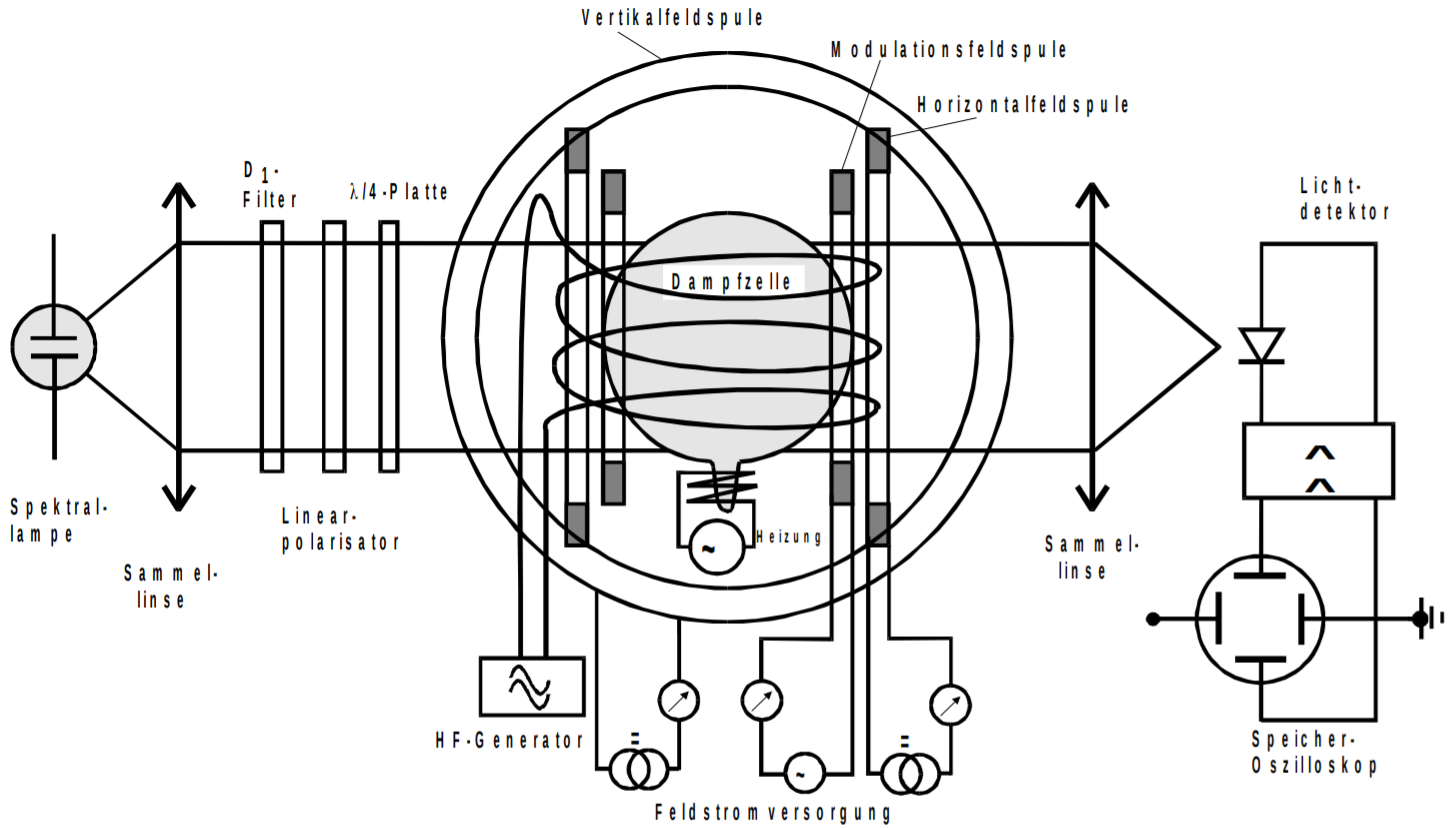
\includegraphics[width=0.6\linewidth]{data/Aufbau.png}
	\caption{Schematische Darstellung des verwendeten Versuchsaufbaus.}
	\label{fig:Aufbau}
\end{figure}

\noindent
Das Licht stammt aus einer Rubidium-Spektrallampe. Es wird zunächst durch eine Sammellinse fokussiert und
durchquert anschließend einen D$_1$-Filter, der es auf Licht mit der Wellenlänge $\lambda = 794,8 \si{\nano\metre}$ reduziert. Danach wird das Licht durch zwei weitere
Filter zunächst linear polarisiert und anschließend, durch eine $\frac{\lambda}{4}$-Platte, rechtszirkular polarisiert. Nachdem es die Filter durchlaufen hat, trifft das polarisierte
Licht nun auf die Rubidium Dampfzelle. Diese wird extern geheitzt und ist von mehreren Spulen umgeben. Nachdem das Licht die Dampfzelle durchlaufen hat, wird es erneut durch eine Linse
fokussiert und trifft dann auf ein Si-Photoelement, dass Schwankungen der Lichtintensität detektiert.
\newline
Von den drei Helmholtz-Spulenpaaren, die die Dampfzelle umgeben, ist eins vertikal ausgerichtet, um den vertikalen Anteil des Erdmagnetfeldes auszugleichen. Die beiden anderen Spulenpaare
sind horizontal ausgerichtet. Eins von beiden ist ein Sweep-Spulenpaar und das andere ein RF-Spulenpaar.


\section{Durchführung}
\label{sec:Durchführung}

Bevor die Messungen beginnen können, muss zunächst die Messapparatur justiert werden. Dafür werden die Sammellinsen so platziert, dass der Ausschlag am Lichtdetektor maximal wird.
Dann wird der Tisch, auf dem die Apparatur steht, so ausgerichtet, dass der Lichtstrrahl parallel oder antiparallel zur horizontalen Komponente des Erdmagnetfeldes ist.
Die vertikale Komponente wird dann durch das vertikale Helmholtz-Spulenpaar ausgeglichen. Dieses wird eingestellt indem der Peak, der durch einen Einbruch der Transparenz
der Rubidiumdampfzelle bei Abwesenheit eines Magnetfelds hervorgerufene wird, durch variieren der Feldstärke auf eine minimale Breite gebracht wird. 
\newline \newline
Im Anschluss kann die eigentliche Messung der Resonanzstellen der beiden Isotope beginnen. Hierzu wird die RF-Spule zunächst auf $100\, \si{\kilo\hertz}$ eingestellt und im
Laufe des Versuches, in Schritten von $100\, \si{\kilo\hertz}$, auf bis zu $1\,\si{\mega\hertz}$ erhöht. Dabei werden für jede Frequenz jeweils die beiden Resonanzwerte der
Feldstärke für die zwei Isotope ermittelt. Dabei ist es für höhere Frequenzen nötig, ein zusätzliches horizontales Feld hinzuzuschalten.
